%%%%%%%%%%%%%%%%%%%%%%%%%%%%%%%%%%%%%%%%%%%%%%%%%%%%%%%%%%%%%%%%%%%%%%%%%%%%%%%
%
% Filename: ira-analysis.tex
% Author:   David Oniani
% Modified: September 21, 2019
%  _         _____   __  __
% | |    __ |_   _|__\ \/ /
% | |   / _` || |/ _ \\  /
% | |__| (_| || |  __//  \
% |_____\__,_||_|\___/_/\_\
%
%%%%%%%%%%%%%%%%%%%%%%%%%%%%%%%%%%%%%%%%%%%%%%%%%%%%%%%%%%%%%%%%%%%%%%%%%%%%%%%

%%%%%%%%%%%%%%%%%%%%%%%%%%%%%%%%%%%%%%%%%%%%%%%%%%%%%%%%%%%%%%%%%%%%%%%%%%%%%%%
% Document definition
%%%%%%%%%%%%%%%%%%%%%%%%%%%%%%%%%%%%%%%%%%%%%%%%%%%%%%%%%%%%%%%%%%%%%%%%%%%%%%%

\documentclass[11pt]{article}

%%%%%%%%%%%%%%%%%%%%%%%%%%%%%%%%%%%%%%%%%%%%%%%%%%%%%%%%%%%%%%%%%%%%%%%%%%%%%%%
% Packages and related settings
%%%%%%%%%%%%%%%%%%%%%%%%%%%%%%%%%%%%%%%%%%%%%%%%%%%%%%%%%%%%%%%%%%%%%%%%%%%%%%%

% Global, document-wide settings
\usepackage[margin=1in]{geometry}
\usepackage[utf8]{inputenc}
\usepackage[english]{babel}

% Bibliography and references
\usepackage[backend=biber]{biblatex}
\addbibresource{$BIB}

% Math and alignment
\usepackage{multicol}
\usepackage{bookmark}
\usepackage{adjustbox}
\usepackage{braket}
\usepackage{mathtools}
\usepackage{amsmath}
\usepackage{amssymb}
\usepackage{amsthm}
\usepackage{amsfonts}
\usepackage{algorithmic}

% Graphics
\usepackage{pgfplots}
\pgfplotsset{compat=1.16}
\usepackage{tikz}
\usetikzlibrary{cd, arrows, decorations.markings}
\usepackage{graphicx}
\usepackage{rotating}
\usepackage{pst-solides3d}
\usepackage{xcolor}

% Fancy stuff
\usepackage{fancyhdr}
\usepackage{tocloft}
\usepackage{caption}
\usepackage{soul}
\usepackage{textcomp}
\usepackage{wasysym}
\usepackage[cache=false]{minted}
\usepackage{csquotes}
\usepackage{hyperref}

%%%%%%%%%%%%%%%%%%%%%%%%%%%%%%%%%%%%%%%%%%%%%%%%%%%%%%%%%%%%%%%%%%%%%%%%%%%%%%%
% Mathematican operations and operators
%%%%%%%%%%%%%%%%%%%%%%%%%%%%%%%%%%%%%%%%%%%%%%%%%%%%%%%%%%%%%%%%%%%%%%%%%%%%%%%

% Sets and related operators
\newcommand{\nats}{\mathbb{N}}                   % Natural numbers
\newcommand{\pnats}{\mathbb{N}^+}                % Positive natural numbers

\newcommand{\ints}{\mathbb{Z}}                   % Integers
\newcommand{\pints}{\mathbb{Z}^+}                % Positive integers
\newcommand{\nints}{\mathbb{Z}^-}                % Negative integers

\newcommand{\rats}{\mathbb{Q}}                   % Rational numbers
\newcommand{\prats}{\mathbb{Q}^+}                % Positive rational numbers
\newcommand{\nrats}{\mathbb{Q}^-}                % Negative rational numbers

\newcommand{\reals}{\mathbb{R}}                  % Real numbers
\newcommand{\preals}{\mathbb{R}^+}               % Positive real numbers
\newcommand{\nreals}{\mathbb{R}^-}               % Negative real numbers

\newcommand{\irrats}{\mathbb{I}}                 % Irrational numbers

\newcommand{\pset}{\mathcal{P}}                  % Powerset
\newcommand{\card}{\abs}                         % Cardinality
\newcommand{\topology}{\mathcal{T}}              % Topology
\newcommand{\basis}{\mathcal{B}}                 % Basis
\newcommand{\oldemptyset}{\emptyset}             % Old empty set
\renewcommand{\emptyset}{\varnothing}            % New and nice empty set

% Other operators
\DeclarePairedDelimiter\abs{\lvert}{\rvert}      % Absolute value
\DeclarePairedDelimiter\ceil{\lceil}{\rceil}     % Ceiling
\DeclarePairedDelimiter\floor{\lfloor}{\rfloor}  % Floor

%%%%%%%%%%%%%%%%%%%%%%%%%%%%%%%%%%%%%%%%%%%%%%%%%%%%%%%%%%%%%%%%%%%%%%%%%%%%%%%
% Command definitions and redefinitions
%%%%%%%%%%%%%%%%%%%%%%%%%%%%%%%%%%%%%%%%%%%%%%%%%%%%%%%%%%%%%%%%%%%%%%%%%%%%%%%

% New commands
\newcommand{\rarr}{\rightarrow}                        % Leftarrow
\newcommand{\larr}{\leftarrow}                         % Rightarrow
\newcommand\und[1]{\underline{\smash{#1}}}             % Nice-looking underline

% Renewed commands
\renewcommand{\headrulewidth}{0.5pt}                   % Header rule width
\renewcommand{\footrulewidth}{0pt}                     % Footer rule width
\renewcommand{\baselinestretch}{1.5}                   % Line spacing is 1.5
\renewcommand{\cftsecleader}{\cftdotfill{\cftdotsep}}  % Dots for ToC sections

% Rename "Contents" to "Table of Contents"
\addto\captionsenglish{% Replace "english" with the language used
  \renewcommand{\contentsname}%
    {\textbf{Table of Contents}}}%

% Filling the space for centering the title of the table of contents
\renewcommand{\cfttoctitlefont}{\hspace*{\fill}\Large}
\renewcommand{\cftaftertoctitle}{\hspace*{\fill}}

%%%%%%%%%%%%%%%%%%%%%%%%%%%%%%%%%%%%%%%%%%%%%%%%%%%%%%%%%%%%%%%%%%%%%%%%%%%%%%%
% Miscellaneous
%%%%%%%%%%%%%%%%%%%%%%%%%%%%%%%%%%%%%%%%%%%%%%%%%%%%%%%%%%%%%%%%%%%%%%%%%%%%%%%

% Setting stuff
\setlength{\parindent}{0pt}  % Remove indentations from paragraphs
\frenchspacing               % Get rid of large spaces after dots
\pagestyle{fancy}            % This allows to do fancy headers and footers
\fancyhf{}                   % No additional page numbering (or other stuff)
\cfoot{\thepage}             % Display page number at the bottom, in the center

% PDF information and nice-looking urls
\hypersetup{%
  pdfauthor  = {David Oniani},
  pdftitle   = {Textual and Statistical Analysis of Russian IRA Facebook Posts},
  pdfsubject = {Statistics, Authorship Attribution, Visual Persuasion},
  colorlinks = true,
  linkcolor  = {blue!50!black},
  citecolor  = {blue!50!black},
  urlcolor   = {blue!50!black}
}

% Put a centered header of a footnote size on the top of each page
\chead{\footnotesize{\MakeUppercase{Textual and Statistical Analysis of Russian IRA Facebook Posts}}}

% Definition environment
\theoremstyle{definition}
\newtheorem*{definition}{Definition}

%%%%%%%%%%%%%%%%%%%%%%%%%%%%%%%%%%%%%%%%%%%%%%%%%%%%%%%%%%%%%%%%%%%%%%%%%%%%%%%
% Author(s), title, and date
%%%%%%%%%%%%%%%%%%%%%%%%%%%%%%%%%%%%%%%%%%%%%%%%%%%%%%%%%%%%%%%%%%%%%%%%%%%%%%%

% Author(s)
\author{David Oniani\\
        Luther College\\
        \href{mailto:oniada01@luther.edu}{oniada01@luther.edu}}

% Title
\title{\textbf{Textual and Statistical Analysis of Russian IRA Facebook Posts}\\
      \small \textsuperscript{*}The paper is written in the scope of a student-faculty collaborative\\
                                summer research with professor Richard K. Merritt.}

% Date
\date{Month Day, Year}

%%%%%%%%%%%%%%%%%%%%%%%%%%%%%%%%%%%%%%%%%%%%%%%%%%%%%%%%%%%%%%%%%%%%%%%%%%%%%%%
% Beginning of the document
%%%%%%%%%%%%%%%%%%%%%%%%%%%%%%%%%%%%%%%%%%%%%%%%%%%%%%%%%%%%%%%%%%%%%%%%%%%%%%%

\begin{document}
\maketitle

%%%%%%%%%%%%%%%%%%%%%%%%%%%%%%%%%%%%%%%%%%%%%%%%%%%%%%%%%%%%%%%%%%%%%%%%%%%%%%%
% Abstract
%%%%%%%%%%%%%%%%%%%%%%%%%%%%%%%%%%%%%%%%%%%%%%%%%%%%%%%%%%%%%%%%%%%%%%%%%%%%%%%

\begin{abstract}
\addcontentsline{toc}{section}{Abstract}

\noindent The 2016 United States Presidential Election was targeted by an
unprecedented intelligence and influence campaign. Arising out of Russian
so-called Internet Research Agency (IRA), it sought to sow discord and attack
the fissures of the United States with the ultimate goal of swaying the
election results.~\cite{ira2016}~\cite{ira2016data} Recently, some of the
IRA-backed Facebook advertisements were released by The United States House
Permanent Select Committee on Intelligence.  All of the advertisements are in
the PDF format. We have scraped the PDF files and present the results obtained
by textual and statistical analysis of the above-mentioned data. Authorship
attribution and sentiment analysis tests were also performed.~\footnote{Please
note that this paper does not discuss neither social, nor political implications
of these events, but attempts to explore the methods of persuasion that were
employed in this influence campaign.}~\cite{ira2016csvdata} We have also made
the data publicly available for other researchers and/or interested people in
a much nicer and easier-to-manipulate CSV format.
\end{abstract}

%%%%%%%%%%%%%%%%%%%%%%%%%%%%%%%%%%%%%%%%%%%%%%%%%%%%%%%%%%%%%%%%%%%%%%%%%%%%%%%
% Table of Contents
%%%%%%%%%%%%%%%%%%%%%%%%%%%%%%%%%%%%%%%%%%%%%%%%%%%%%%%%%%%%%%%%%%%%%%%%%%%%%%%

\newpage
\tableofcontents
\newpage

%%%%%%%%%%%%%%%%%%%%%%%%%%%%%%%%%%%%%%%%%%%%%%%%%%%%%%%%%%%%%%%%%%%%%%%%%%%%%%%
% Data and Preparation
%%%%%%%%%%%%%%%%%%%%%%%%%%%%%%%%%%%%%%%%%%%%%%%%%%%%%%%%%%%%%%%%%%%%%%%%%%%%%%%

\section*{\centering Data Preparation}
\addcontentsline{toc}{section}{Data Preparation}

The data was scraped from~\cite{ira2016data} more than 3500 Russian IRA
Facebook posts made publicly available in the PDF format by the House
Intelligence Committee. We used the free and open-source Python library
~\cite{pdftotext} \texttt{pdftotext} to scrape the data. Many CSV files were
formatted in a way that it was hard for \texttt{pdftotext} to scrape it
correctly. Because of this, we have manually reviewed most of the CSV files
for validity.~\cite{ira2016csvdata} All the CSV files have been made publicly
available.

%%%%%%%%%%%%%%%%%%%%%%%%%%%%%%%%%%%%%%%%%%%%%%%%%%%%%%%%%%%%%%%%%%%%%%%%%%%%%%%
% General Statistics
%%%%%%%%%%%%%%%%%%%%%%%%%%%%%%%%%%%%%%%%%%%%%%%%%%%%%%%%%%%%%%%%%%%%%%%%%%%%%%%

\section*{\centering General Statistics}
\addcontentsline{toc}{section}{General Statistics}
The distribution of posts over all three years shows us a bimodal distribution
with two peaks in 2016 Quarter 2 and 2016 Quarter 4. Given the fact that the US
Presidential Elections were held in 2016 Quarter 4, it is surprising that the
second quarter had the most of the Facebook ads in it.

\begin{figure}[H]
\centering
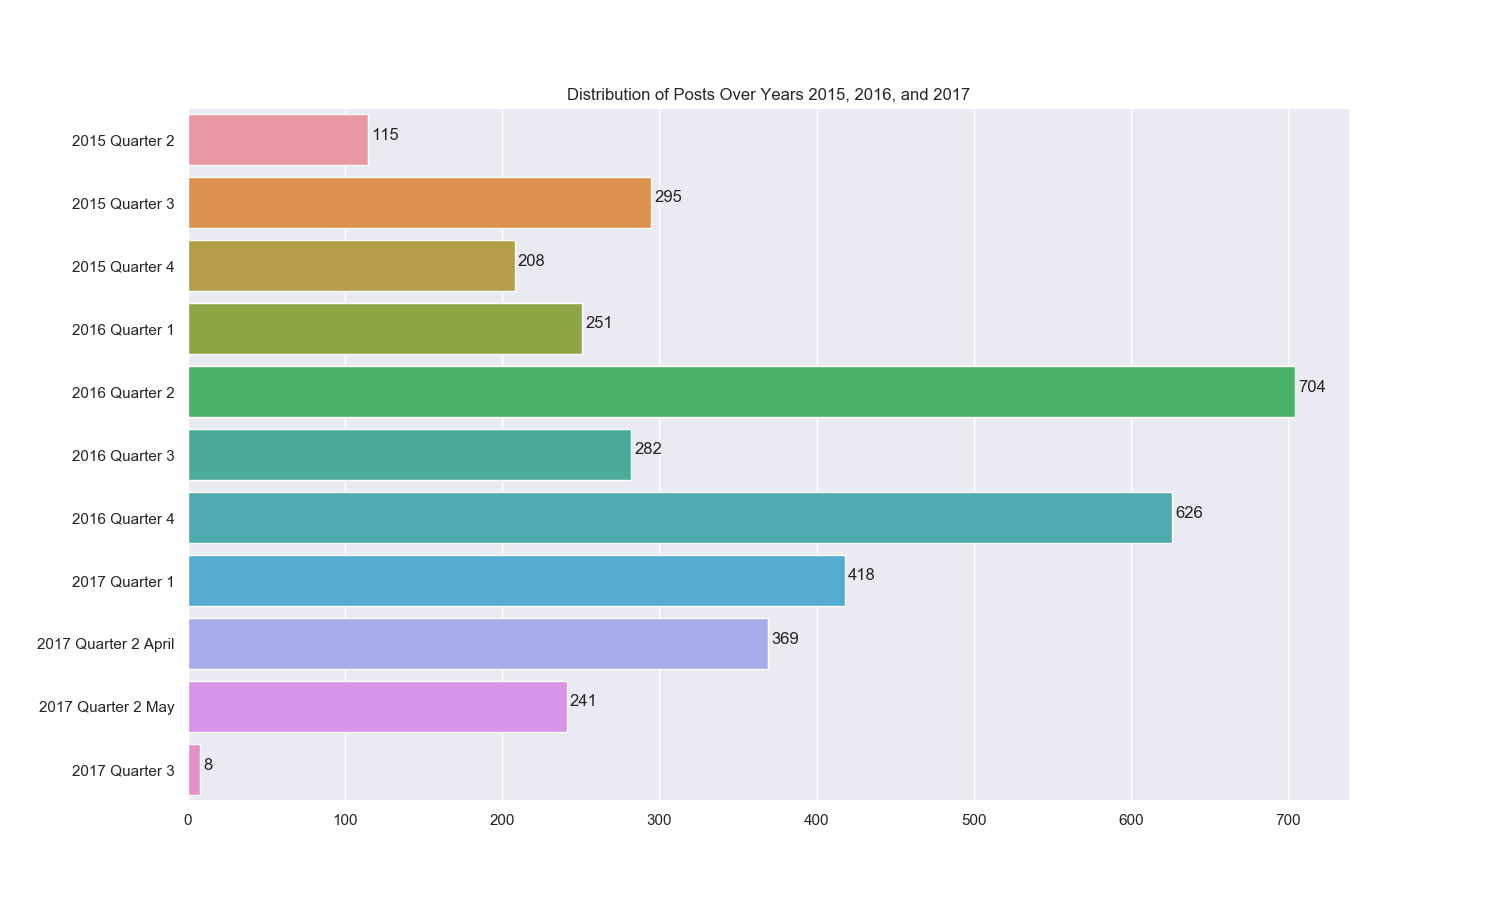
\includegraphics[width=\textwidth]{../visualization/barchart-plots/barchart_distribution_of_posts.png}
\caption*{Distribution of Posts Over Years 2015, 2016, and 2017.}
\end{figure}

When it comes the money spent on ads, however, the fourth quarter of 2016 is,
by far, the one on which IRA spent the most money on. It is also interesting
that most of of the money was payed in Russian Rubles with two exceptions in
2016 quarter 3 and 2017 quarter 1 where they have spent \$74.000 and \$35.330
respectively.

\begin{figure}[H]
\centering
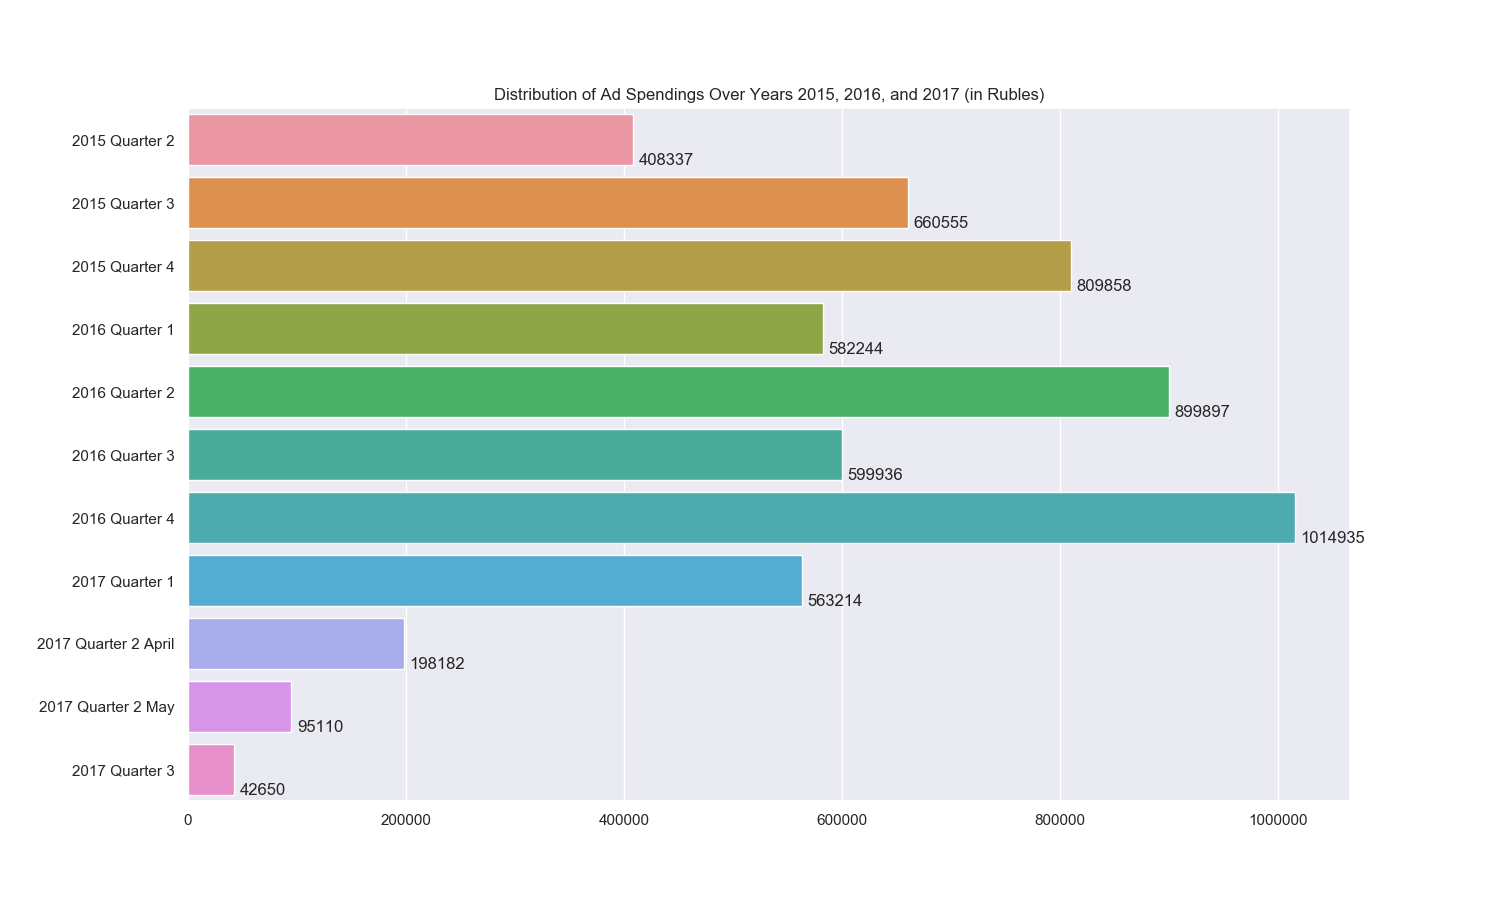
\includegraphics[width=\textwidth]{../visualization/barchart-plots/barchart_ad_spend_RU_distribution.png}
\caption*{Distribution of Ad Spendings Over Years 2015, 2016, and 2017 (in Rubles).}
\end{figure}

%%%%%%%%%%%%%%%%%%%%%%%%%%%%%%%%%%%%%%%%%%%%%%%%%%%%%%%%%%%%%%%%%%%%%%%%%%%%%%%
% Textual Analysis
%%%%%%%%%%%%%%%%%%%%%%%%%%%%%%%%%%%%%%%%%%%%%%%%%%%%%%%%%%%%%%%%%%%%%%%%%%%%%%%

\section*{\centering Textual Analysis}
\addcontentsline{toc}{section}{Textual Analysis}

\subsection*{\centering Common Words}
\addcontentsline{toc}{subsection}{Common Words}

Lorem ipsum dolor sit amet, consectetur adipiscing elit.
Aenean porta purus et sem gravida rutrum.
Maecenas blandit nulla ac luctus tempus.
Nam finibus posuere ante, et lacinia massa vestibulum sit amet.
Nulla velit arcu, efficitur quis turpis nec, sollicitudin lobortis nisi.
Vivamus ut diam ut eros faucibus fringilla.
Suspendisse pellentesque magna nec velit tristique sollicitudin.
Morbi ultrices nec augue et molestie.
Nam sapien ante, ullamcorper elementum convallis id, faucibus in lectus.
Fusce pellentesque mollis velit efficitur porta.
Sed finibus ligula quam, et lacinia velit posuere auctor.
Donec ligula lorem, dictum nec lectus in, vehicula tincidunt massa.
In hac habitasse platea dictumst.

\begin{figure}[H]
\centering
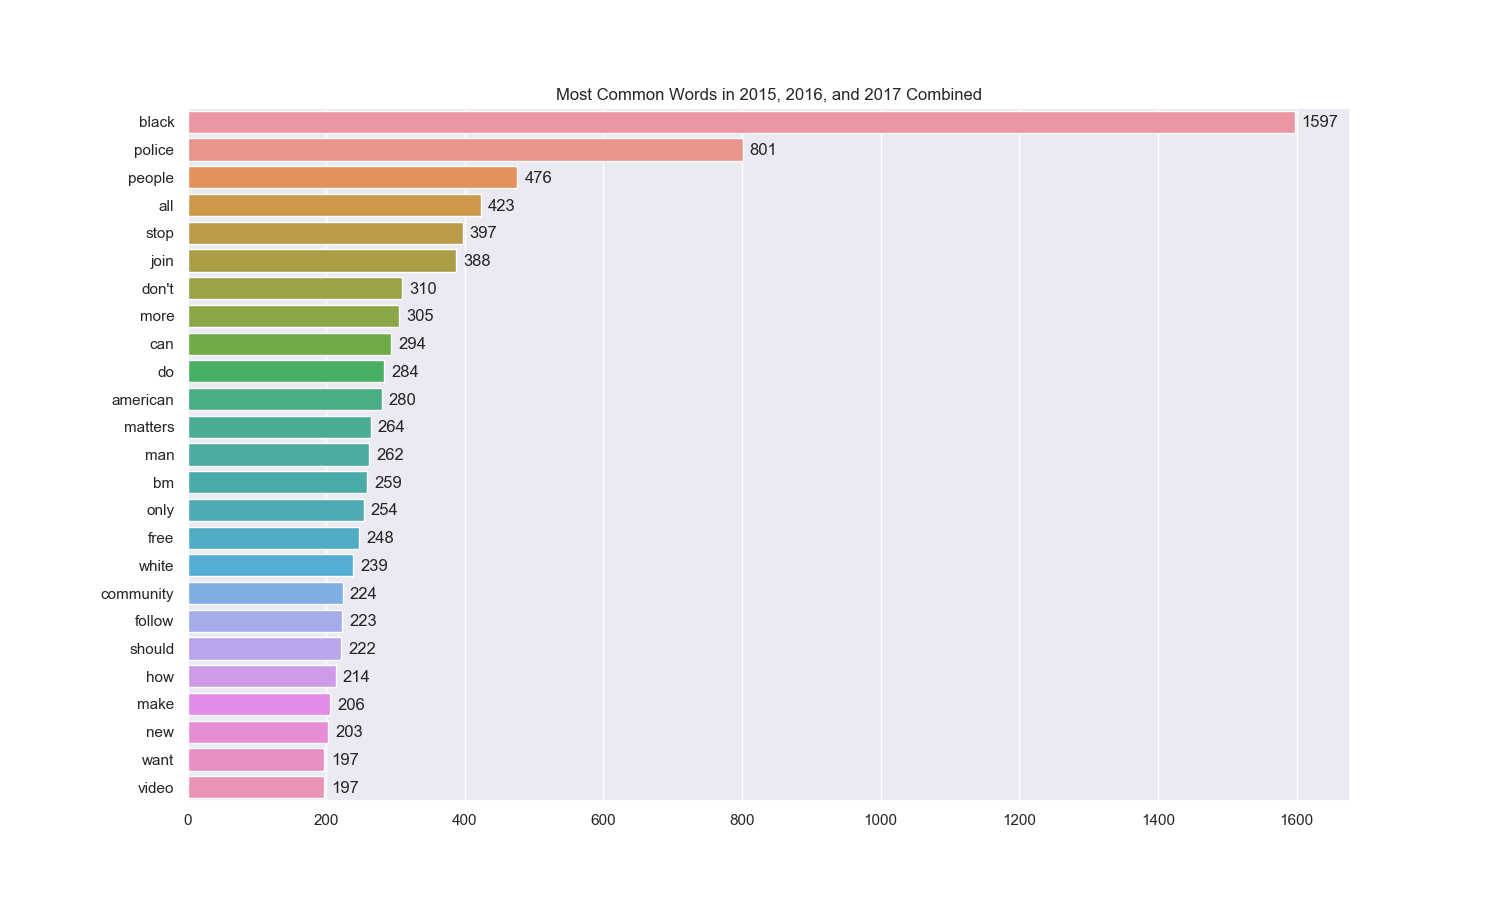
\includegraphics[width=\textwidth]{../visualization/barchart-plots/barchart_word_counts.png}
\caption*{Figure.}
\end{figure}

%%%%%%%%%%%%%%%%%%%%%%%%%%%%%%%%%%%%%%%%%%%%%%%%%%%%%%%%%%%%%%%%%%%%%%%%%%%%%%%
% Sentiment Analysis
%%%%%%%%%%%%%%%%%%%%%%%%%%%%%%%%%%%%%%%%%%%%%%%%%%%%%%%%%%%%%%%%%%%%%%%%%%%%%%%

\subsubsection*{\centering Common Words}
\addcontentsline{toc}{subsection}{Sentiment Analysis}
For the sentiment analysis purposes, we used \texttt{python}'s \texttt{TextBlob}
library. Suprisingly, out of all Facebook posts with \texttt{Ad Text}, 1643 were
positive, 900 negative, and 933 neutral leaving the overall tone of the posts
positive.

\begin{center}
\begin{tabular}{ |p{3cm}|p{3cm}|p{3cm}|p{3cm}|  }
 \hline
 \multicolumn{4}{|c|}{Analyzing Negativity} \\
 \hline
 Subjectivity Level & Year 2015 & Year 2016 & Year 2017\\
 \hline
 1.0  & 154 & 562 & 176\\
 0.75 & 150 & 547 & 169\\
 0.5  & 123 & 405 & 120\\
 0.25 & 15  & 81  & 22 \\
 0.15 & 5   & 33  & 10 \\
 0.1  & 2   & 11  & 6  \\
 0.05 & 1   & 5   & 2  \\
 \hline
\end{tabular}
\end{center}


%%%%%%%%%%%%%%%%%%%%%%%%%%%%%%%%%%%%%%%%%%%%%%%%%%%%%%%%%%%%%%%%%%%%%%%%%%%%%%%
% Authorship Attribution
%%%%%%%%%%%%%%%%%%%%%%%%%%%%%%%%%%%%%%%%%%%%%%%%%%%%%%%%%%%%%%%%%%%%%%%%%%%%%%%

\subsubsection*{\centering Authorship Attribution}
\addcontentsline{toc}{subsection}{Authorship Attribution}

Lorem ipsum dolor sit amet, consectetur adipiscing elit.
Aenean porta purus et sem gravida rutrum.
Maecenas blandit nulla ac luctus tempus.
Nam finibus posuere ante, et lacinia massa vestibulum sit amet.
Nulla velit arcu, efficitur quis turpis nec, sollicitudin lobortis nisi.
Vivamus ut diam ut eros faucibus fringilla.
Suspendisse pellentesque magna nec velit tristique sollicitudin.
Morbi ultrices nec augue et molestie.
Nam sapien ante, ullamcorper elementum convallis id, faucibus in lectus.
Fusce pellentesque mollis velit efficitur porta.
Sed finibus ligula quam, et lacinia velit posuere auctor.
Donec ligula lorem, dictum nec lectus in, vehicula tincidunt massa.
In hac habitasse platea dictumst.

%%%%%%%%%%%%%%%%%%%%%%%%%%%%%%%%%%%%%%%%%%%%%%%%%%%%%%%%%%%%%%%%%%%%%%%%%%%%%%%
% Bibliography and References
%%%%%%%%%%%%%%%%%%%%%%%%%%%%%%%%%%%%%%%%%%%%%%%%%%%%%%%%%%%%%%%%%%%%%%%%%%%%%%%

\newpage

\begin{center}
\printbibliography[heading=bibintoc]
\end{center}

%%%%%%%%%%%%%%%%%%%%%%%%%%%%%%%%%%%%%%%%%%%%%%%%%%%%%%%%%%%%%%%%%%%%%%%%%%%%%%%
% The end of the document
%%%%%%%%%%%%%%%%%%%%%%%%%%%%%%%%%%%%%%%%%%%%%%%%%%%%%%%%%%%%%%%%%%%%%%%%%%%%%%%

\end{document}
